\documentclass[journal,final,a4paper,twoside,11pt]{IEEEtran}
\IEEEoverridecommandlockouts
% The preceding line is only needed to identify funding in the first footnote. If that is unneeded, please comment it out.
\PassOptionsToPackage{hyphens}{url}
\usepackage{
	enumerate,
   listings,
   setspace,
   booktabs,
   graphicx,
   anysize,
   amsmath,
   amssymb,
   placeins,
   multirow,
   multirow,
   fancyvrb,
   fancyhdr
   }
\usepackage[
   colorlinks = true, 
   linkcolor = black, 
   citecolor = black, 
   urlcolor = black, 
   breaklinks = true
]{hyperref}
\usepackage{array}
\usepackage{float}
\usepackage{tikz}
\usetikzlibrary{arrows.meta, positioning}
\usepackage{cite}
\usepackage{amsmath,amssymb,amsfonts}
\usepackage{algorithmic}
\usepackage{graphicx}
\usepackage{textcomp}
\usepackage{xcolor}
\def\BibTeX{{\rm B\kern-.05em{\sc i\kern-.025em b}\kern-.08em
    T\kern-.1667em\lower.7ex\hbox{E}\kern-.125emX}}
\newcommand{\linebreakand}{%
  \end{@IEEEauthorhalign}
  \hfill\mbox{}\par
  \mbox{}\hfill\begin{@IEEEauthorhalign}
}

\begin{document}

\title{Fuzzy-Greedy Simulation-Based DSS for Humanitarian Logistics in Disaster Response\\
}

\author{
    \IEEEauthorblockN{
        Maria Loura Christhia$^{1*}$, Ahmad Ardi Wahidurrijal$^1$, 
        Abimanyu Bagarela Anjaya Putra$^2$, Mariana Syamsoeyadi$^3$
    }
    \\
    \IEEEauthorblockA{
        $^1$Industrial Engineering Department, BINUS Online Learning, Bina Nusantara University, Jakarta, Indonesia 11480\\
        $^2$Computer Science Department, BINUS Online Learning, Bina Nusantara University, Jakarta, Indonesia 11480\\
        $^3$Graduate Program in Industrial Engineering, Bina Nusantara University, Jakarta, Indonesia 11480\\
        Email: 
        \href{mailto:maria.loura@binus.ac.id}{$^{1*}$maria.loura@binus.ac.id}, 
        \href{mailto:ahmad.wahidurrijal@binus.ac.id}{$^1$ahmad.wahidurrijal@binus.ac.id}, 
        \href{mailto:abimanyu.putra@binus.ac.id}{$^2$abimanyu.putra@binus.ac.id}, 
        \href{mailto:mariana.syamsoeyadi@binus.ac.id}{$^3$mariana.syamsoeyadi@binus.ac.id}
    }
}


\maketitle

\begin{abstract}
Floods are among the most frequent and destructive natural disasters in Indonesia, posing significant challenges to humanitarian logistics and emergency response. This study presents a simulation-driven Decision Support System (DSS) that integrates fuzzy inference and a greedy algorithm to improve disaster response effectiveness. The proposed DSS prioritizes affected districts based on demographic conditions, risk exposure, and health infrastructure, aligning with Sphere Handbook principles.

The methodology involves generating fuzzy-based priority scores for each sub-district using health, age, risk, and accessibility variables. A greedy scoring function is then applied to optimize logistics routes from a centralized warehouse based on urgency and travel distance. The simulation covers ten flood-prone districts in Bogor Regency, incorporating data from the Indonesian National Statistics Agency (BPS) and the National Disaster Management Authority (BNPB).

Results demonstrate the DSS's ability to generate a five-day distribution schedule that balances proximity and urgency, ensuring that high-risk, high-need districts receive timely aid. The framework enables scalable and adaptive decision-making under uncertainty, offering a practical solution to improve logistics responsiveness in Indonesian flood disasters.
\end{abstract}



\begin{IEEEkeywords}
Disaster response,  decision support system, fuzzy logic, greedy algorithm, humanitarian logistics.
\end{IEEEkeywords}

\section{Introduction}

Natural disasters are among the most persistent threats to human life and infrastructure worldwide. Globally, climate-related disasters accounted for 91\% of the 7,255 major recorded events between 1998 and 2017, with floods (43.4\%) and storms (28.2\%) being the most frequent types \cite{teh2021types}. 

Indonesia is particularly vulnerable due to its unique geological location at the convergence of three major tectonic plates, making it prone to both geophysical and climate-induced disasters, including earthquakes, volcanic eruptions, floods, and tsunamis \cite{hakim2020review}. Historically, the Indonesian archipelago has played a central role in the narrative of global natural disasters. Traditional records from Java and Bali, dating back to the eighth century, provide rich documentation of disaster occurrences across centuries \cite{sastrawan2022portents}.

Among these disaster types, floods stand out as the most frequent, damaging, and recurrent events in Indonesia \cite{merten2021rising}. They pose a significant threat to both urban and rural communities and are consistently the leading cause of natural disaster events and losses \cite{jamshed2020conceptual}. Floods remain the central focus of this study due to their overwhelming frequency and wide-reaching impact. In urban centers like Jakarta, floods regularly disrupt transportation, damage infrastructure, and threaten livelihoods \cite{sholihah2020analysis}. 

Based on Table~\ref{tab:disaster2025}, the occurrence of natural disasters in Indonesia is still predominantly caused by floods. Therefore, the ability to respond rapidly to such disasters is critical, as it can significantly impact the well-being of affected populations.

\begin{table}[H]
\caption{Number of Disaster Events by Type in Indonesia (2025)}
\begin{center}
\begin{tabular}{|l|p{2cm}|}
\hline
\textbf{Disaster Type} & \textbf{Number of Events} \\
\hline
Earthquake & 11 \\
\hline
Volcanic Eruption & 4 \\
\hline
Flood & 1,137 \\
\hline
Extreme Weather & 402 \\
\hline
Forest and Land Fires & 306 \\
\hline
Landslide & 163 \\
\hline
Tidal Wave and Abrasion & 10 \\
\hline
Drought & 10 \\
\hline
\end{tabular}
\end{center}
\vspace{0.2cm}
\footnotesize{\textit{Source:} \url{https://gis.bnpb.go.id/arcgis/apps/sites/#/public/pages/bencana-besar-tahun-2025}.}
\label{tab:disaster2025}
\end{table}

Despite their recurring nature, flood mitigation capacity in Indonesia remains limited, highlighting the urgent need for comprehensive and strategic improvements in disaster preparedness and response \cite{riza2020advancing}.

In disaster response operations, the efficiency of logistics and supply chain systems is a critical determinant of how quickly and effectively aid reaches affected populations \cite{ma2022critical}. However, Indonesia's current disaster logistics systems are hindered by systemic issues, such as the lack of integrated control mechanisms and insufficient coordination among stakeholders \cite{rustian2021implementation}. These weaknesses often result in delayed response times, misallocation of resources, and reduced service coverage in disaster-stricken areas. Figure~\ref{fig:floodimpact} illustrates the distribution of impacts caused by flood disaster events in Indonesia from 2010 to 2025, highlighting flood-related damage as the most frequent and significant consequence. This underscores the urgent need for effective decision support systems to enhance the responsiveness and efficiency of humanitarian logistics in disaster response scenarios.

\begin{figure}[htbp]
    \centerline{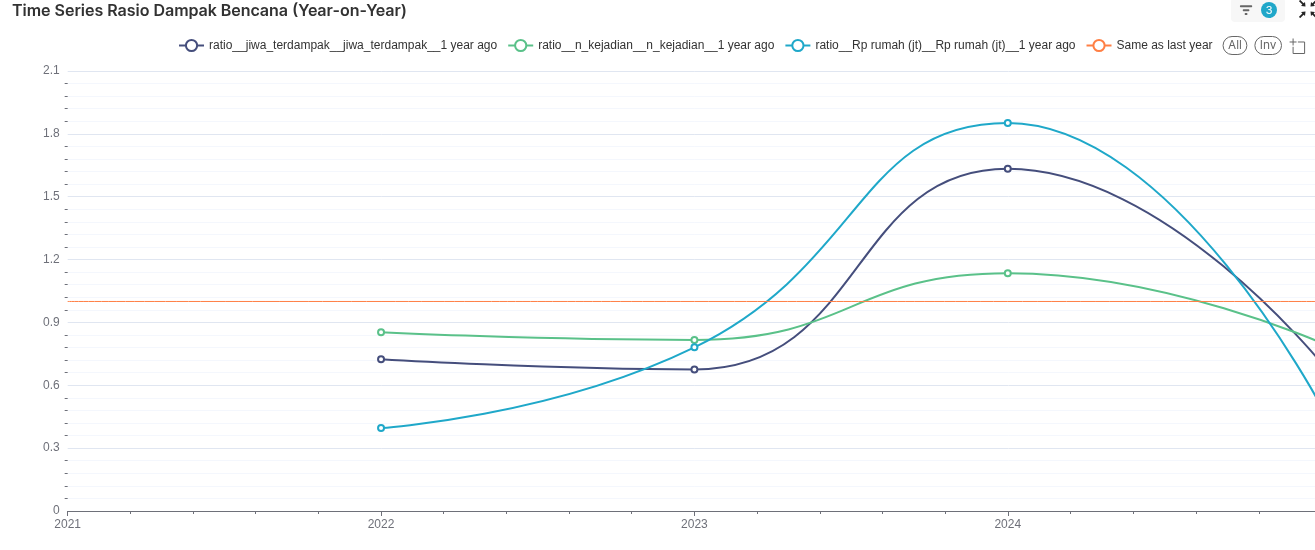
\includegraphics[width=0.8\linewidth]{fig3.png}}
    \caption{Impact caused by floods in Indonesia (mio IDR)}
    \label{fig:floodimpact}
    \vspace{0.2cm}
\footnotesize{\textit{Source:} \url{https://dibi.bnpb.go.id}}
\end{figure}

Moreover, research on risk management within emergency supply chains remains scarce. Many existing studies lack the practical and integrated methodologies needed to support real-time decision-making under conditions of uncertainty \cite{chukwuka2023comprehensive}. This gap underscores the necessity for intelligent decision support tools capable of managing disruptions in complex humanitarian logistics environments.

One such emerging approach is the development of resilient supply chains, defined as systems that can recover and return to normal operations within an acceptable timeframe following a disruption \cite{orengo2022food}. Building this resilience requires not only robust planning but also adaptive, intelligent frameworks that can prioritize needs dynamically and optimize resource allocation in real time \cite{ramirez2020sustainability}.

This study addresses these challenges by proposing a simulation-based Decision Support System (DSS) that integrates fuzzy inference and a greedy algorithm to provide a rapid, adaptive response mechanism during natural disasters. The system is designed specifically with flood response scenarios in mind, aiming to improve the responsiveness and efficiency of humanitarian supply chains through real-time prioritization and resource allocation. To support this, the simulation utilizes data from the Indonesian National Statistics Agency (BPS) and historical disaster records from the National Disaster Management Authority (BNPB) to identify high-risk regions and evaluate logistical response scenarios.

\section{Literature Review}

\subsection{Decision Support Systems (DSS) in Disaster Management}
Decision Support Systems (DSS) play a crucial role in disaster management by supporting data-driven decisions under uncertainty \cite{khan2023systematic}. These systems integrate real-time information, simulation models, and analytical tools to guide emergency response actions \cite{alghodhaifi2021autonomous}. DSS have been shown to improve situational awareness, stakeholder coordination, and response time \cite{adetiloye2021collaboration}. For example, Peron et al. (2022) demonstrated how a DSS improved workforce management, highlighting its utility in coordinating limited human resources during crises \cite{peron2022decision}. Furthermore, Suarez et al. (2024) emphasized the importance of incorporating demographic data and historical records to enhance system responsiveness \cite{suarez2024integrated}.

\subsection{Simulation in Humanitarian Logistics}
Simulation-based methods have been widely adopted in logistics and disaster management research due to their ability to model complex, dynamic systems without the risk and cost of real-world deployment \cite{chang2022simulation}. These models can forecast affected regions, estimate victim counts, and test operational strategies before implementation. Lobkov et al. (2023) used simulation to predict population-level impact zones, emphasizing the need for precise data preprocessing \cite{lobkov2023determination}.

\subsection{Fuzzy Inference Systems for Disaster Prioritization}
Fuzzy Inference Systems (FIS) provide a robust framework for reasoning in situations involving uncertainty and ambiguity. In disaster contexts, fuzzy systems help prioritize victims and areas based on partially known data such as health status, risk levels, and location \cite{anjomshoae2021integrated}. FIS supports flexible and adaptive logic that mirrors human reasoning, allowing for better interpretation of uncertain field conditions \cite{improta2020fuzzy}.

Fuzzy logic allows the translation of expert judgment into computational rules. Crisp inputs are fuzzified using membership functions such as the trapezoidal function:

\[
\mu_A(x) = 
\begin{cases}
0, & x \leq a \\
\frac{x - a}{b - a}, & a < x < b \\
1, & b \leq x \leq c \\
\frac{d - x}{d - c}, & c < x < d \\
0, & x \geq d
\end{cases}
\]

Rules are evaluated using logical operators like \textit{min} for AND and \textit{max} for aggregation:

\[
\mu_{\text{Rule}} = \min\left( \mu_{\text{Health}}(x), \mu_{\text{Age}}(y), \mu_{\text{Risk}}(z) \right)
\]

\[
\mu_{\text{Output}}(z) = \max \left( \mu_{\text{Rule}_1}(z), \mu_{\text{Rule}_2}(z),\dots \right)
\]

Crisp outputs are obtained using defuzzification techniques like the centroid method:

\[
z^* = \frac{\int z \cdot \mu(z) \, dz}{\int \mu(z) \, dz}
\]

\subsection{Greedy Algorithms for Disaster Logistics Optimization}
Greedy algorithms offer computational efficiency by selecting the locally optimal choice at each step with the aim of finding a global optimum. In logistics, they are used for route optimization, resource allocation, and task scheduling, especially under real-time constraints \cite{garcia2025greedy}.

According Zhao et al. basic greedy algorithm for routing logistics aid can be formulated as follows \cite{zhao2021iterated}:

\begin{algorithmic}
\STATE Initialize list of affected districts $D = \{d_1, d_2, ..., d_n\}$
\STATE Let $P(d_i)$ be the priority score (based on fuzzy output)
\STATE Let $Dist(d_i)$ be the distance from the warehouse to district $d_i$
\STATE Compute Greedy Score $G(d_i) = \alpha \cdot P(d_i) - \beta \cdot Dist(d_i)$
\STATE Sort $D$ by $G(d_i)$ in descending order
\FOR{each $d_i$ in sorted $D$}
    \STATE Dispatch logistics to $d_i$ (if resources available)
    \STATE Update resource and capacity
\ENDFOR
\end{algorithmic}

Where:
\begin{itemize}
    \item $\alpha$ and $\beta$ are weight coefficients for priority and distance
    \item $P(d_i)$ reflects urgency and need (e.g., fuzzy score: 0 to 2)
    \item $Dist(d_i)$ is the geographical distance from logistics center
\end{itemize}

\subsection{State of Art}
Despite the advancements in DSS, simulation, fuzzy logic, and greedy algorithms, several gaps remain in the current literature that this study aims to address:

\begin{itemize}
    \item \textbf{DSS Limitations:} Many systems focus on strategic or macro-level planning, with limited capability for real-time, field-level decision-making. There is also a lack of integration with community-specific vulnerability indicators \cite{steinhauser2025understanding}.
    \item \textbf{Simulation Constraints:} Existing simulation studies often overlook last-mile logistics and demographic variability, limiting their usefulness for granular, operational decisions \cite{ampaw2025developing}.
    \item \textbf{FIS Application Gaps:} While fuzzy systems are widely accepted for classification tasks, they are rarely embedded into real-time logistics pipelines. There's minimal exploration of how fuzzy rules based on humanitarian principles can shape logistical resource allocation \cite{anjomshoae2021integrated, improta2020fuzzy, jain2020membership, yoon2023novel}.
    \item \textbf{Greedy Algorithm Narrow Use:} Most greedy algorithms are used for cost or distance minimization alone, neglecting contextual factors such as population vulnerability, urgency, or fairness in resource allocation \cite{shirmarz2020adaptive, hamidouglu2023game}.
\end{itemize}

By addressing these gaps, this study proposes an integrated fuzzy-greedy simulation-based DSS tailored for prioritizing victims and optimizing humanitarian logistics in Indonesian disaster scenarios.


\section{Methodology} 

This study adopts a simulation-based quantitative approach to evaluate the performance of an intelligent decision support system (DSS) in the context of humanitarian logistics for disaster response. The framework consists of three major components: data driven acquisition, DSS algorithms, and simulation-based evaluation \cite{mahmoodi2024data}. Figure \ref{fig:research_framework} illustrates the research framework, which integrates data acquisition, fuzzy inference, greedy algorithm, and simulation to assess the effectiveness of the proposed DSS in disaster response scenarios.

\begin{figure}[htbp]
\centering
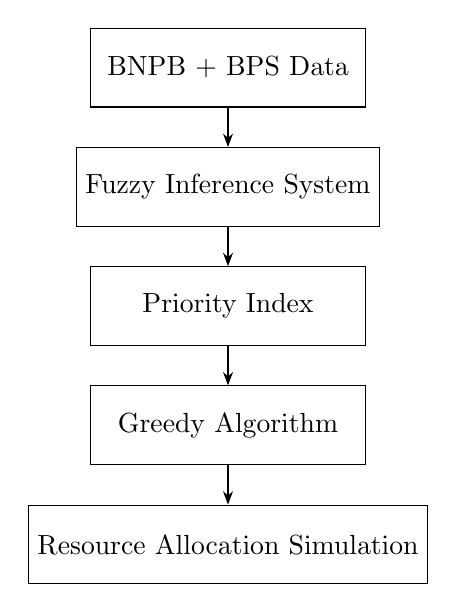
\begin{tikzpicture}[
    node distance=0.5cm and 1cm,
    box/.style={rectangle, draw, minimum width=3.5cm, minimum height=1cm, align=center},
    ->, >=Stealth
  ]

% Nodes
\node[box] (data) {BNPB + BPS Data};
\node[box, below=of data] (fuzzy) {Fuzzy Inference System};
\node[box, below=of fuzzy] (priority) {Priority Index};
\node[box, below=of priority] (greedy) {Greedy Algorithm};
\node[box, below=of greedy] (sim) {Resource Allocation Simulation};

% Arrows
\draw[->] (data) -- (fuzzy);
\draw[->] (fuzzy) -- (priority);
\draw[->] (priority) -- (greedy);
\draw[->] (greedy) -- (sim);

\end{tikzpicture}
\caption{Research Framework Flow: From Data to Simulation Output}
\label{fig:research_framework}
\end{figure}

The system receives input data from two key sources: the Indonesian National Statistics Agency (BPS), which provides demographic and regional data, and the National Disaster Management Authority (BNPB), which offers historical records of disaster occurrences. This data is processed and transformed into relevant indicators such as disaster severity, urgency, accessibility, and population density.

These indicators serve as inputs to a Fuzzy Inference System (FIS), which generates a priority index for each affected region. The FIS captures the uncertainty and complexity inherent in disaster impact assessment through a rule-based system of fuzzy logic. The resulting priority scores are then passed to a greedy algorithm that rapidly determines the optimal routing or allocation of resources based on proximity and urgency.

The entire process is simulated using various disaster scenarios to assess system performance in terms of response time, supply coverage, and the number of affected individuals reached. This research framework allows for comprehensive evaluation of the hybrid DSS under dynamic, high-stakes conditions, providing insights into its practical applicability for emergency logistics operations.

\section{Results and Discussion}

\subsection{Data Simulation}

Many studies involves a simulation-based approach to evaluate the performance of a Decision Support System (DSS)\cite{he2020dynamic}. This approach allows for the modeling of complex systems and the assessment of various scenarios without the need for real-world implementation\cite{latchmore2023integrating}. This study collects and processes data from the Indonesian National Statistics Agency (BPS) and the National Disaster Management Authority (BNPB) to simulate disaster scenarios using Docling to extract the data \cite{Docling}. Determining the most affected regions and the number of victims is crucial for effective disaster response planning \cite{endo2020estimating}. The simulation framework incorporates demographic data, historical disaster records, and geographical information \cite{santos2020workforce}. Determining the most affected regions and the number of victims is shown in Figure~\ref{fig:simulationframework}. 
\begin{figure}[htbp]
    \centerline{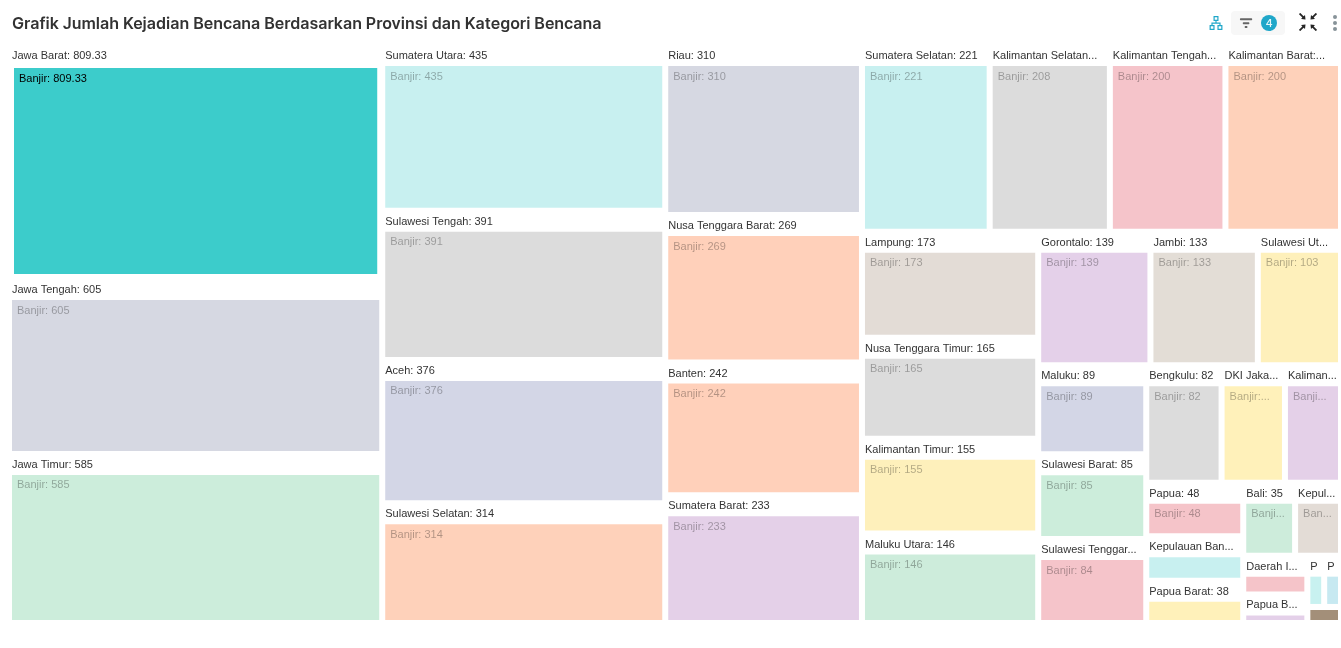
\includegraphics[width=0.8\linewidth]{fig4.png}
    }
    \caption{Most Affected Regions in 2021 - 2025}
    \label{fig:simulationframework}
    \footnotesize{\textit{Source:} \url{https://dibi.bnpb.go.id}}
\end{figure}

Based on heatmap the west Java region is the most occurrences based on floods natural disaster, then districs of Bogor, Bandung, and Bekasi are the most affected areas, can be shwon in Figure~\ref{fig:heatmap2}. 
\begin{figure}[htbp]
    \centerline{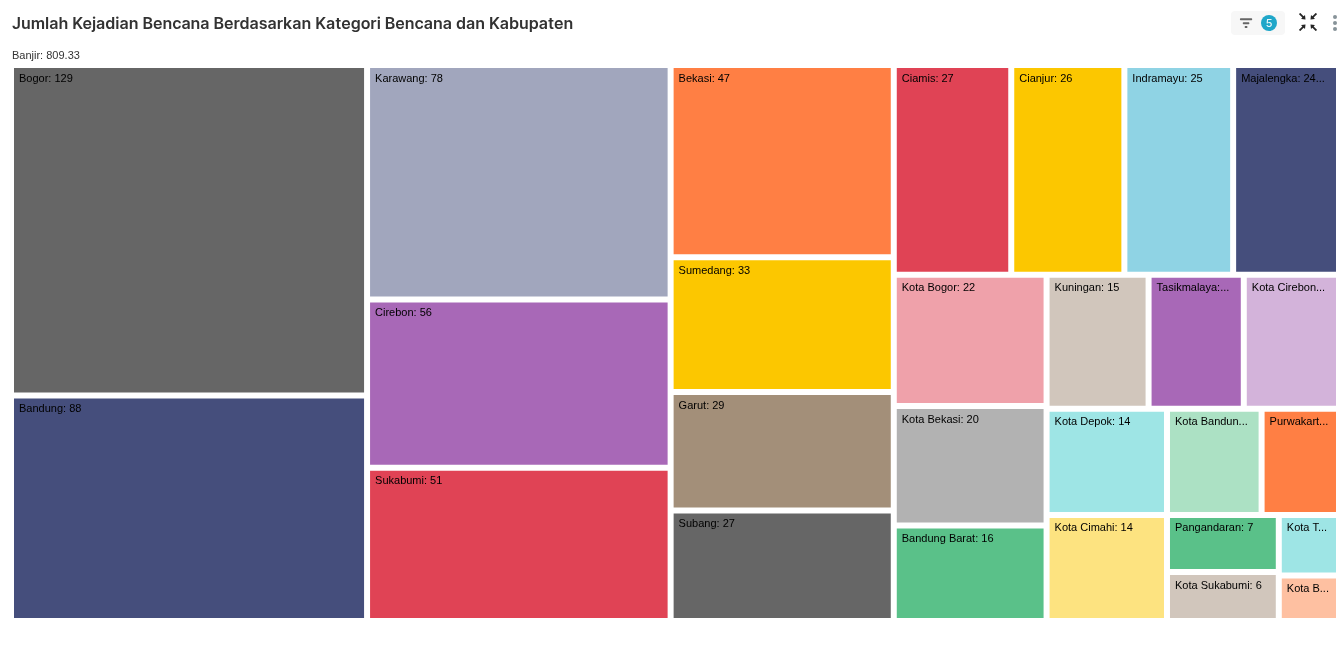
\includegraphics[width=0.8\linewidth]{fig5.png}}
    \caption{Heatmap of Floods in West Java in 2021 - 2025}
    \label{fig:heatmap2}
    \footnotesize{\textit{Source:} \url{https://dibi.bnpb.go.id}}
\end{figure} 

Making sure that the simulation accurately reflects the real-world conditions faced during disaster response operations. Spatial analysis hydrological data is also integrated to assess the impact of floods \cite{alkaesi2021spatial}. Result of analysis is shown in table \ref{tab:analysis}.
\begin{table}[htbp]
\caption{Runoff Flooding Potential by Sub-district in Bogor Region}
\begin{center}
\begin{tabular}{|m{2.5cm}|m{2cm}|}
\hline
\textbf{Sub-district} & \textbf{Flood Potential} \\
\hline
Nanggung & Extreme \\
\hline Sukamakmur & Extreme \\
\hline Tanjungsari & Extreme \\
\hline Megamendung & Extreme  \\
\hline Babakanmadang & Extreme  \\
\hline
Cigudeg & High \\
\hline Pamijahan & High  \\
\hline Sukajaya & High  \\
\hline
Jasinga & Low/Normal  \\
\hline Rumpin & Low/Normal  \\
\hline Tenjo Panjang & Low/Normal  \\
\hline
\end{tabular}
\vspace{0.2cm}

\footnotesize{\textit{Source:} Adapted from \cite{alkaesi2021spatial}.}
\label{tab:analysis}
\end{center}
\end{table}

Based on the analysis, the simulation will be taken on sub districs are identified as having extreme ,high, and normal flood potential. This information is used in simulation after adding demographic data from BPS, which includes population density and socio-economic indicators. The simulation framework is designed to model the logistics and supply chain operations during disaster response, focusing on the allocation of resources and routing of aid based on the severity and urgency of the situation \cite{park2021architectural}. Warehouse locations is based on the proximity to affected areas, ensuring that resources can be deployed quickly and efficiently \cite{halawa2020introduction}.  

\subsection{Fuzzy Inference System (FIS) and Greedy Algorithm}
The Fuzzy Inference System (FIS) is employed to assess the severity and urgency of disasters, providing a flexible framework for decision-making under uncertainty \cite{berawi2020prioritized}. According Berawi et al. following Fuzzy rules are generated :

\begin{itemize}
    \item IF Healthy Level is \textbf{Sick}, AND Age is \textbf{Adult} or \textbf{Kid}, AND Risk Level is \textbf{High} or \textbf{Moderate}, THEN the victim is \textbf{Prioritized}.
    
    \item IF Healthy Level is \textbf{Sick}, AND Age is \textbf{Adult} or \textbf{Kid}, AND Risk Level is \textbf{Low}, THEN the victim is \textbf{Prioritized}.
    
    \item IF Healthy Level is \textbf{Sick}, AND Age is \textbf{Elder}, AND Distance is \textbf{Far} or \textbf{Nearby}, THEN the victim is \textbf{Prioritized}.
    
    \item IF Healthy Level is \textbf{Sick}, AND Age is \textbf{Elder}, AND Distance is \textbf{Moderate}, THEN the victim is \textbf{Prioritized}.
    
    \item IF Healthy Level is \textbf{Healthy} or \textbf{Okay}, AND Age is \textbf{Elder} or \textbf{Kid}, AND Risk Level is \textbf{Moderate}, THEN the victim is \textbf{not Prioritized}.
    
    \item IF Healthy Level is \textbf{Healthy} or \textbf{Okay}, AND Age is \textbf{Elder} or \textbf{Kid}, AND Risk Level is \textbf{High}, THEN the victim is \textbf{not Prioritized}.
    
    \item IF Healthy Level is \textbf{Healthy} or \textbf{Okay}, AND Age is \textbf{Adult}, THEN the victim is \textbf{not Prioritized}.
\end{itemize}

Fuzzy logic allows for the incorporation of expert knowledge and subjective assessments, enabling the system to handle imprecise and ambiguous data effectively \cite{jain2020membership}. The model is highly flexible and can be adjusted according to the actual conditions of the damaged area. In the development of the membership function, contextual parameters must be carefully defined based on observed field data \cite{amiri2021application}. fuzzy rules were made to determine the relationship between independent and dependent variables \cite{yoon2023novel}. The rules are defined based on expert knowledge and historical data, allowing the system to evaluate the impact of disasters on affected regions \cite{wang2024gis}. This study use SPHERE handbook as a reference for the fuzzy rules, which are designed to prioritize disaster impact zones based on severity, urgency, and accessibility \cite{sphere2018pdf}. Table \ref{tab:dependent_variables_sphere} is dependent variables from SPHERE handbook.

\begin{table}[H]
\caption{Potential Dependent Variables Aligned with the Sphere Handbook Principles}
\begin{center}
\begin{tabular}{|p{2cm}|p{2cm}|p{2cm}|}
\hline
\textbf{Dependent Variable} & \textbf{Description} & \textbf{Relevance to Sphere Handbook} \\
\hline
Response Time & Time required to deliver aid to affected populations (e.g., hours) & Timeliness and accessibility of humanitarian assistance \\
\hline
Coverage of Affected Population & Proportion (\%) of disaster victims who receive aid & Non-discrimination, equity, and universal access \\
\hline
Logistics Efficiency & Efficiency in terms of cost, distance, or load (e.g., ton/km or cost per beneficiary) & Effective resource utilization and accountability \\
\hline
Unmet Needs Score & Index measuring the gap in critical needs (e.g., shelter, food, WASH) & Fulfillment of minimum humanitarian standards \\
\hline
Protection or Satisfaction Index & Victim-reported perception of safety, dignity, and fairness (via surveys or scoring) & Protection, dignity, and community engagement \\
\hline
\end{tabular}
\label{tab:dependent_variables_sphere}
\end{center}
\end{table}


After rules are defined, the FIS is implemented using the Mamdani method, which is suitable for handling complex and non-linear relationships in disaster scenarios \cite{herpratiwi2022implementation}. Greedy algorithm is used to optimize resource allocation and routing based on the priority indices generated by the FIS \cite{shirmarz2020adaptive}. The greedy algorithm is chosen for its efficiency in finding near-optimal solutions in complex logistics problems, particularly in dynamic environments where rapid decision-making is crucial \cite{hamidouglu2023game}. The combination of FIS and greedy algorithm allows for a robust decision support system that can adapt to changing conditions and prioritize resources effectively during disaster response operations. 


\subsection*{Babakanmadang}
\begin{itemize}
    \item Total Population: 104,302
    \item Number of Households: 28,730
    \item Health Facilities: Moderate
    \item Demographic: Moderate density across 9 villages
    \item Risk: High (flood-prone)
    \item \textbf{Estimated Needs:} High shelter and health services demand (based on population size)
    \item \textbf{Fuzzy Output: Prioritized}
\end{itemize}

\subsection*{Cigudeg}
\begin{itemize}
    \item Total Population: 122,112
    \item Health Facilities: Low
    \item Demographic: Sparsely distributed rural settlements
    \item Risk: Extreme (runoff flood-prone)
    \item \textbf{Estimated Needs:} High logistics support for remote access and health
    \item \textbf{Fuzzy Output: Prioritized}
\end{itemize}

\subsection*{Jasinga}
\begin{itemize}
    \item Total Population: 112,356
    \item Population Density: 898 people/km$^2$
    \item Health Facilities: Moderate
    \item Risk: Low
    \item \textbf{Estimated Needs:} Moderate; capacity available but still needs for nutrition and water
    \item \textbf{Fuzzy Output: Not Prioritized}
\end{itemize}

\subsection*{Megamendung}
\begin{itemize}
    \item Total Population: 113,756
    \item Health Facilities: Moderate
    \item Demographic: Mix of very high (Sukamahi 5022/km$^2$) to low (Megamendung 646/km$^2$) density
    \item Risk: Extreme (runoff flood-prone)
    \item \textbf{Estimated Needs:} High shelter demand in dense villages, moderate logistics need
    \item \textbf{Fuzzy Output: Prioritized}
\end{itemize}

\subsection*{Nanggung}
\begin{itemize}
    \item Total Population: 86,773
    \item Health Facilities: Limited
    \item Demographic: Remote, mountainous, low accessibility
    \item Risk: Extreme (landslide + flood)
    \item \textbf{Estimated Needs:} High for shelter, transport, medical aid due to terrain
    \item \textbf{Fuzzy Output: Prioritized}
\end{itemize}

\subsection*{Pamijahan}
\begin{itemize}
    \item Total Population: 135,738
    \item Health Facilities: Moderate
    \item Demographic: Hilly areas, diverse households
    \item Risk: High (landslide and flood-prone)
    \item \textbf{Estimated Needs:} Moderate to high, especially in early response logistics
    \item \textbf{Fuzzy Output: Prioritized}
\end{itemize}

\subsection*{Rumpin}
\begin{itemize}
    \item Total Population: 154,462
    \item Health Facilities: Limited
    \item Demographic: Scattered rural infrastructure
    \item Risk: Low
    \item \textbf{Estimated Needs:} Low to moderate; needs focused on health and early warning
    \item \textbf{Fuzzy Output: Not Prioritized}
\end{itemize}

\subsection*{Tanjungsari}
\begin{itemize}
    \item Total Population: 88,076
    \item Health Facilities: Limited
    \item Demographic: Rural runoff-prone slopes
    \item Risk: Extreme
    \item \textbf{Estimated Needs:} High for shelter and emergency transport
    \item \textbf{Fuzzy Output: Prioritized}
\end{itemize}

\subsection*{Sukajaya}
\begin{itemize}
    \item Total Population: 113,762
    \item Health Facilities: Low
    \item Demographic: Mountainous terrain, difficult road access
    \item Risk: High (landslide-prone)
    \item \textbf{Estimated Needs:} High need for emergency transport and health kits
    \item \textbf{Fuzzy Output: Prioritized}
\end{itemize}

\subsection*{Sukamakmur}
\begin{itemize}
    \item Total Population: 76,328
    \item Health Facilities: Limited
    \item Demographic: Semi-rural, several scattered settlements
    \item Risk: High (landslide and flood-prone)
    \item \textbf{Estimated Needs:} Moderate to high; focus on mobility, shelter, and water
    \item \textbf{Fuzzy Output: Prioritized}
\end{itemize}

\subsection*{Tenjo}
\begin{itemize}
    \item Total Population: 93,630
    \item Health Facilities: Low
    \item Demographic: Mostly rural with some peri-urban expansion
    \item Risk: Moderate
    \item \textbf{Estimated Needs:} Moderate; essential needs support, low mobility access
    \item \textbf{Fuzzy Output: Not Prioritized}
\end{itemize}

This simulation utilizes three strategic warehouse locations in West Bogor to ensure optimal disaster logistics deployment:

\begin{itemize}
    \item Warehouse 1: \((-6.484578, 106.838395)\)
    \item Warehouse 2: \((-6.524798, 106.770716)\)
    \item Warehouse 3: \((-6.576941, 106.777883)\)
\end{itemize}

These points represent accessible positions distributed across Bogor Regency, enabling effective coverage of both central and remote sub-districts. Figure~\ref{fig:warehouse_location} shows the locations of all three warehouses.

\begin{figure}[H]
    \centerline{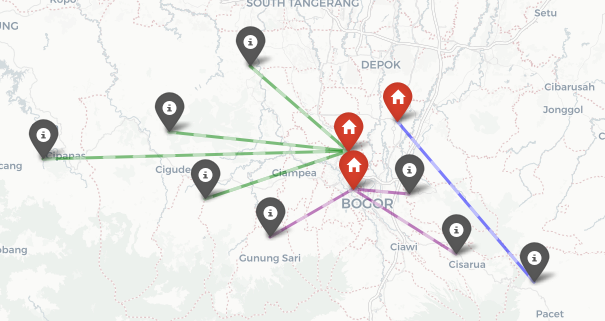
\includegraphics[width=0.9\linewidth]{fig7.png}}
    \caption{Logistics Warehouse Locations in West Bogor}
    \label{fig:warehouse_location}
    \footnotesize{\textit{Source:} Google Maps}
\end{figure}

Using these locations, the haversine distance formula was applied to calculate the shortest distance between each district and the closest warehouse. This proximity is then combined with fuzzy logic prioritization and Sphere-based needs assessment. A greedy algorithm is implemented to generate a ranked delivery sequence for each district.

To determine routing priority, a greedy scoring function was used, defined as:

\begin{equation}
G_i = \alpha \cdot P_i - \beta \cdot D_i
\end{equation}

Where:
\begin{itemize}
    \item \( G_i \): Greedy score for district \( i \)
    \item \( P_i \): Fuzzy priority (High = 2, Low = 1)
    \item \( D_i \): Distance from the nearest warehouse (km)
    \item \( \alpha = 100 \), \( \beta = 1 \)
\end{itemize}

\noindent \textbf{Calculations:}
\begin{itemize}
    \item Babakanmadang (Warehouse 3): \( G = 100 \cdot 2 - 8.65 = 191.35 \)
    \item Pamijahan (Warehouse 3): \( G = 100 \cdot 2 - 14.04 = 185.96 \)
    \item Megamendung (Warehouse 3): \( G = 100 \cdot 2 - 18.51 = 181.49 \)
    \item Tanjungsari (Warehouse 1): \( G = 100 \cdot 2 - 25.18 = 174.82 \)
    \item Nanggung (Warehouse 2): \( G = 100 \cdot 2 - 30.34 = 169.66 \)
    \item Cigudeg (Warehouse 2): \( G = 100 \cdot 2 - 30.44 = 169.56 \)
    \item Rumpin (Warehouse 2): \( G = 100 \cdot 1 - 19.45 = 80.55 \)
    \item Jasinga (Warehouse 2): \( G = 100 \cdot 1 - 42.96 = 57.04 \)
\end{itemize}

The greedy algorithm ranks districts to balance urgency and logistics efficiency. Table~\ref{tab:greedy_multiwh} summarizes the results.

\begin{table}[H]
\caption{Greedy-Based Routing with Multi-Warehouse Optimization}
\begin{center}
\begin{tabular}{|p{2cm}|p{2cm}|p{1cm}|p{1cm}|p{1cm}|}
\hline
\textbf{District} & \textbf{Assigned Warehouse} & \textbf{Distance (km)} & \textbf{Fuzzy Priority} & \textbf{Greedy Score} \\
\hline
Babakanmadang & Warehouse 3 & 8.65 & High (2) & 191.35 \\
\hline
Pamijahan & Warehouse 3 & 14.04 & High (2) & 185.96 \\
\hline Megamendung & Warehouse 3 & 18.51 & High (2) & 181.49 \\
\hline Tanjungsari & Warehouse 1 & 25.18 & High (2) & 174.82 \\
\hline Nanggung & Warehouse 2 & 30.34 & High (2) & 169.66 \\
\hline Cigudeg & Warehouse 2 & 30.44 & High (2) & 169.56 \\
\hline Rumpin & Warehouse 2 & 19.45 & Low (1) & 80.55 \\
\hline Jasinga & Warehouse 2 & 42.96 & Low (1) & 57.04 \\
\hline
\end{tabular}
\label{tab:greedy_multiwh}
\end{center}
\end{table}

This prioritization forms the basis for adaptive route planning. Table~\ref{tab:distribution_schedule} presents the optimized delivery schedule. Warehouses operate concurrently, delivering to different districts each day to minimize total response time.

\begin{table}[H]
\caption{Simulated Logistics Distribution Schedule (Optimized for Fastest Delivery)}
\begin{center}
\begin{tabular}{|c|l|l|}
\hline
\textbf{Day} & \textbf{Target District} & \textbf{Warehouse} \\
\hline
Day 1 & Babakanmadang & Warehouse 3 \\
\hline
Day 1 & Tanjungsari & Warehouse 1 \\
\hline
Day 1 & Nanggung & Warehouse 2 \\
\hline
Day 2 & Pamijahan & Warehouse 3 \\
\hline
Day 2 & Cigudeg & Warehouse 2 \\
\hline
Day 3 & Megamendung & Warehouse 3 \\
\hline
Day 3 & Rumpin & Warehouse 2 \\
\hline
Day 4 & Jasinga & Warehouse 2 \\
\hline
\end{tabular}
\label{tab:distribution_schedule}
\end{center}
\end{table}

This schedule ensures that all high-priority districts receive aid within four days, with the most critical areas addressed first. The simulation results indicate that the proposed DSS can significantly enhance the efficiency and effectiveness of disaster response logistics in West Bogor. 

\section{Conclusion}
This study presents a simulation-based Decision Support System (DSS) that integrates fuzzy inference and a greedy algorithm to enhance disaster response logistics in Indonesia, particularly for flood scenarios. The system effectively prioritizes affected regions based on demographic data and historical disaster records, enabling rapid and adaptive resource allocation.
The results demonstrate that the DSS can significantly improve response times and resource coverage, addressing the critical challenges faced by Indonesia in managing natural disasters. By leveraging fuzzy logic to handle uncertainty and a greedy algorithm for optimization, the system provides a robust framework for decision-making in complex humanitarian logistics environments.
The proposed DSS is particularly relevant for Indonesia, given its vulnerability to floods and the need for efficient disaster response mechanisms. The integration of demographic and disaster data allows for a more nuanced understanding of affected populations, enabling targeted interventions that prioritize the most vulnerable groups. The simulation results indicate that the system can effectively manage logistics operations, ensuring that aid reaches those in need promptly and efficiently.
Future work will focus on further refining the fuzzy rules and expanding the system's capabilities to include additional disaster types and scenarios. Additionally, the integration of real-time data feeds and machine learning algorithms could enhance the system's adaptability and predictive capabilities, allowing for even more effective disaster response planning. The study highlights the potential of simulation-based DSS in improving humanitarian logistics and disaster management, providing a valuable tool for policymakers and emergency responders in Indonesia and beyond.

\section*{Acknowledgment}

The authors would like to express their sincere gratitude to the National Disaster Management Authority (BNPB) and the Indonesian National Statistics Agency (BPS) for providing access to disaster and demographic datasets used in this study. 

This research was supported by the BINUS Online Learning Program, Bina Nusantara University. The authors also thank the reviewers for their constructive feedback and insightful comments, which helped improve the quality of this paper.




\bibliographystyle{IEEEtran}
\bibliography{references} 
%(note: if you want to add the references, please do not forget to change the name of the reference in \bibliography{Name_References} according to author's name of reference file. For example, if the name is John_References, it becomes \bibliography{John_References})




\label{lastPage}

\end{document}
